\begin{figure}[t]
\centering
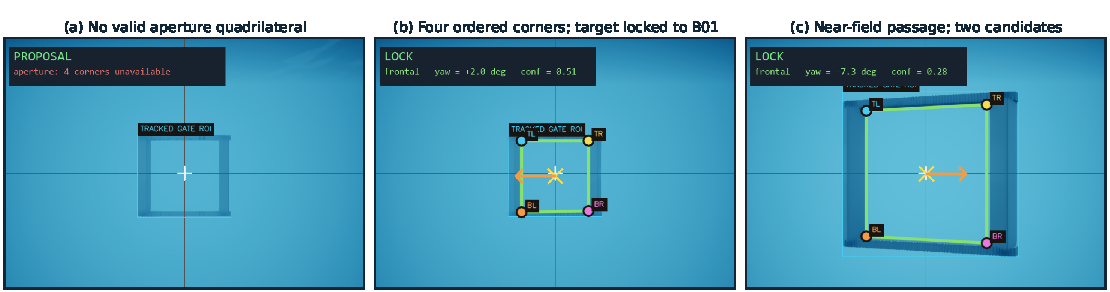
\includegraphics[width=\linewidth]{figures/generated/gate_perception_panels.pdf}
\caption{Onboard gate perception in the native HoloOcean simulator backend, one representative state per
official circuit. Each panel shows the forward-camera frame with the detector's
own overlays: the tracked aperture region, the four canonically ordered corners
(TL, TR, BR, BL), the image-centre crosshair, the estimated gate centre and the
image error vector of \eqref{eq:vision_center} that the visual servo drives to
zero. (a)~Mixed Endurance: a target is detected but no valid aperture
quadrilateral is available, so the front end degrades to the centre-only
estimate and reports an unknown orientation. (b)~Horseshoe Bay: four validated
corners with the target associated to the expected beacon \texttt{B01} at
$4.39$\,m and $-0.0^{\circ}$ bearing, tracker phase \textsc{visual\_align}.
(c)~Vertical Serpent: a near-field passage at $2.25$\,m with two raw candidates,
in which the association of Section~\ref{sec:perception_assoc} retains the
correct target, tracker phase \textsc{verify\_exit}. Nothing shown here is
derived from simulator gate poses or from the referee. Panel chrome from the
interactive viewer has been cropped and its state badge redrawn in English; the
detector overlays and all quoted values are unmodified.}
\label{fig:perception_panels}
\end{figure}
